\documentclass{DOEproposal}
% NSF proposal generation template style file.
% based on latex stylefiles  written by Stefan Llewellyn Smith and
% Sarah Gille, with contributions from other collaborators.
%
% Additions by Ronni Grapenthin, New Mexico Tech.
%
% Obviously it is your responsibility to make sure that everything
% is, in fact, in agreement with the most current NSF Grant 
% Proposal Guide and the respective Program's solicitation! 
% This is all provided `as-is' and no blame or responsibility
% for anything that went wrong will be taken.
%
% Good luck!
%

\usepackage{longtable}
\usepackage[latin1]{inputenc}
\usepackage{latexsym}
\usepackage{amsmath, amsthm, amssymb}
\usepackage{amsfonts}
\usepackage[format=plain,indention=.6cm, font=small, labelfont=bf]{caption}
\usepackage{fancyhdr}
\usepackage[pdftex]{graphicx}
\usepackage[pdftex,
	    colorlinks, 	
	    pdfstartview=FitH,
	    linkcolor=black,
	    citecolor=black,
	    urlcolor=black,
	    filecolor=black
	    ]{hyperref}
\usepackage{lscape}
\usepackage[T1]{fontenc}
\usepackage{floatrow}

%a few commands to highlight issues in the proposal (\TODO, \CHECK, \DummyText)
\RequirePackage{color}
\definecolor{RED}{rgb}{1,0,0}
\definecolor{BLUE}{rgb}{0,0,1}
\definecolor{White}{rgb}{1,1,1}
\providecommand{\TODO}[1]{{\protect\color{red}\noindent {\bf [TODO]}\emph{#1} {\bf [/TODO]}}}
\providecommand{\todo}[1]{{\protect\color{red}\noindent {\bf [TODO]}\emph{#1} {\bf [/TODO]}}}
\providecommand{\CHECK}[1]{{\protect\color{blue} #1 (check) }}
\providecommand{\DummyText}[1]{{\protect\color{white} #1}}

\newcommand{\degrees}{$\!\!$\char23$\!$}

\renewcommand{\refname}{\centerline{References cited}}
\renewcommand{\title}{\noindent {\Large{\bf Here Goes Your Title!}}}



% this handles hanging indents for publications
\def\rrr#1\\{\par
\medskip\hbox{\vbox{\parindent=2em\hsize=6.12in
\hangindent=4em\hangafter=1#1}}}

\def\baselinestretch{1}

%%%%%%%%%%%%%%%%%%%%%%%%%%%%%%%%%%%%%%%
%%%%% Document starts here

\begin{document}

%%%%%%%%%%%%%%%%%%%%%%%%%%%%%%%%%%%%%%%
% A - COVER SHEET: Produced by fastlane, type in information there.

%%%%%%%%%%%%%%%%%%%%%%%%%%%%%%%%%%%%%%%
% B - PROJECT SUMMARY
{\bf \title} \\*[3mm]

{\bf Overview:} Each proposal must contain a summary of the proposed project not more than {\bf one page in length}. The Project
Summary consists of an overview, a statement on the intellectual merit of the proposed activity, and a statement
on the broader impacts of the proposed activity.

The overview includes a description of the activity that would result if the proposal were funded and a statement
of objectives and methods to be employed.  

The Project Summary should be written in the third person, informative to other persons working in
the same or related fields, and, insofar as possible, understandable to a scientifically or technically 
literate lay reader. It should not be an abstract of the proposal.

If the Project Summary contains special characters it may be uploaded as a Supplementary Document.
{\bf Project Summaries submitted as a PDF must be formatted with separate headings for the overview, statement on the
intellectual merit of the proposed activity, and statement on the broader impacts of the proposed activity}. Failure
to include these headings may result in the proposal being returned without review.
Additional instructions for preparation of the Project Summary are available in FastLane.\\

{\bf Intellectual Merit:} The statement on intellectual merit should describe the potential of
the proposed activity to advance knowledge.\\

{\bf Broader Impacts: } The statement on broader impacts should describe the potential of
the proposed activity to benefit society and contribute to the achievement of specific, 
desired societal outcomes.

\renewcommand{\thepage} {B--\arabic{page}}
\newpage

%%%%%%%%%%%%%%%%%%%%%%%%%%%%%%%%%%%%%%%
% C - TABLE OF CONTENTS: Automatically generated by fastlane.


%%%%%%%%%%%%%%%%%%%%%%%%%%%%%%%%%%%%%%%
% D - PROJECT DESCRIPTION

% reset page numbering to 1.  This is helpful, since the text can only
% be 15 pages (unless otherwise specified, see individual solicitations), 
% and reviewers will want to believe we've kept within those limits

\pagenumbering{arabic}
\renewcommand{\thepage} {D--\arabic{page}}

\newpage

\title\\

\section{Introduction}

The Project Description should provide a clear statement of the work to be undertaken and must include:
objectives for the period of the proposed work and expected significance; relation to longer-term goals of the PI's
project; and relation to the present state of knowledge in the field, to work in progress by the PI under other
support and to work in progress elsewhere.

The Project Description should outline the general plan of work, including the broad design of activities to be
undertaken, and, where appropriate, provide a clear description of experimental methods and procedures.
Proposers should address what they want to do, why they want to do it, how they plan to do it, how they will
know if they succeed, and what benefits could accrue if the project is successful. The project activities may be
based on previously established and/or innovative methods and approaches, but in either case must be well
justified. These issues apply to both the technical aspects of the proposal and the way in which the project may
make broader contributions.

The Project Description must contain, as a separate section within the narrative, a section labeled ``Broader
Impacts of the Proposed Work''. This section should provide a discussion of the broader impacts of the proposed
activities. Broader impacts may be accomplished through the research itself, through the activities that are
directly related to specific research projects, or through activities that are supported by, but are complementary to 
the project. NSF values the advancement of scientific knowledge and activities that contribute to the
achievement of societally relevant outcomes. Such outcomes include, but are not limited to: full
participation of women, persons with disabilities, and underrepresented minorities in science, technology, engineering, and
mathematics (STEM); improved STEM education and educator development at any level; increased public
scientific literacy and public engagement with science and technology; improved well-being of individuals in
society; development of a diverse,globally competitive STEM workforce; increased partnerships between
academia, industry, and others; improved national security; increased economic competitiveness of the United
States; and enhanced infrastructure for research and education.

Plans for data management and sharing of the products of research, including preservation, documentation, and
sharing of data, samples, physical collections, curriculum materials and other related research and education
products should be described in the Special Information and Supplementary Documentation section of the
proposal (see GPG Chapter II.C.2.j. for additional instructions for preparation of this section).

\section{Another Section}
Figure~\ref{fig:caption} shows how to make a caption float next to the graphic.

\begin{center}
\begin{figure}[!ht]
\floatbox[{\capbeside\thisfloatsetup{capbesideposition={left,bottom},capbesidewidth=0.25\textwidth}}]{figure}[\FBwidth]
{\caption{\label{fig:caption} Horizontal (blue) and vertical (red) motion of the Japanese GEONET GPS network
with co-seismic (static) motion removed. Shows only S-wave and surface waves \citep[e.g.,][]{Grapenthin2011}.}}
{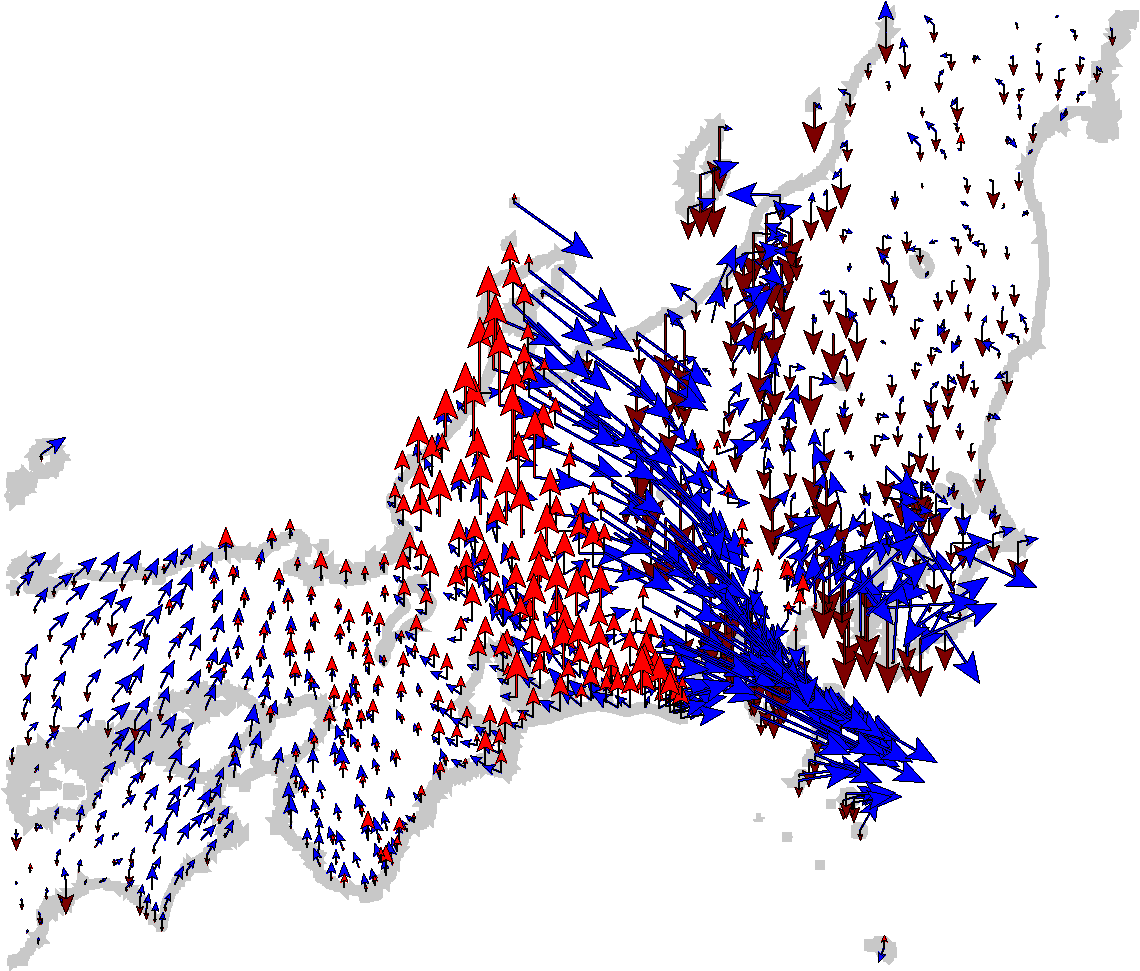
\includegraphics[width=0.75\textwidth]{figure.pdf}}
\end{figure}
\end{center}

\section{Proposed Study}
We'll use the tool by \citet{Grapenthin2014}

\section{Time Line and Management Plan}
How you gonna do it?

\subsection{Subsection}
More text \citep{Grapenthin2006}.

\section{Broader Impacts of the Proposed Work}
Header should be exactly this. 

\section{Results from Prior NSF Support}
If any PI or co-PI identified on the project has received NSF funding (including any current
funding) in the past five years, in formation on the award(s) is required,
irrespective of whether the support was directly related to the proposal or not.
In cases where the PI or co-PI has received more than one award (excluding amendments),
they need only report on the one award most closely related to the proposal. Funding includes not just salary
support, but any funding awarded by NSF. The following information must be provided:\\

\noindent
\emph{\underline{Name of PI}}: NSF-Program (Award Number) ``Title of the Project'' (\$AMOUNT, PERIOD OF SUPPORT). 
{\bf Publications:} List of publications resulting from the NSF award. A complete bibliographic citation for each
publication must be provided either in this section or in the References Cited section of the proposal); if
none, state: ``No publications were produced under this award.'' {\bf Research Products:} evidence of research products 
and their availability, including, but not limited to: data, publications, samples, physical collections, software, 
and models, as described in any Data Management Plan.

%%%%%%%%%%%%%%%%%%%%%%%%%%%%%%%%%%%%%%%
% E - REFERENCES CITED

\newpage
\pagenumbering{arabic}
\renewcommand{\thepage} {E--\arabic{page}}


\bibliography{main}
\bibliographystyle{agufull08}

%%%%%%%%%%%%%%%%%%%%%%%%%%%%%%%%%%%%%%%
% F - BIOGRAPHICAL SKETCHES
% provided separately - see cv_nsf.tex

%%%%%%%%%%%%%%%%%%%%%%%%%%%%%%%%%%%%%%%
% H - CURRENT AND PENDING SUPPORT
% provided separately - see cv_nsf.tex
\newpage
\pagenumbering{arabic}
\renewcommand{\thepage} {F--\arabic{page}}

\section*{Current support}
\begin{tabular}{p{0.25\textwidth}p{0.75\textwidth}}\hline
Agency: 			& NSF						\\
Amount requested: 	& \$X					\\
Period: 			& MM/YYYY-MM/YYYY			\\
Project Title:		& Project Title \\
Effort Committed: 	& X months/year				\\\hline
\end{tabular}

\section*{Pending support}
\begin{tabular}{p{0.25\textwidth}p{0.75\textwidth}}\hline
Agency: 			& NSF						\\
Amount requested: 	& \$X					\\
Period: 			& MM/YYYY-MM/YYYY			\\
Project Title:		& Project Title \\
Effort Committed: 	& X months/year				\\\hline
Agency: 			& USGS						\\
Amount requested: 	& \$X					\\
Period: 			& MM/YYYY-MM/YYYY			\\
Project Title:		& Project Title \\
Effort Committed: 	& X months/year				\\\hline
\end{tabular}


%%%%%%%%%%%%%%%%%%%%%%%%%%%%%%%%%%%%%%%
% G - BUDGET JUSTIFICATION

\newpage
\pagenumbering{arabic}
\renewcommand{\thepage} {G--\arabic{page}}
\noindent{\Large \bf BUDGET JUSTIFICATION}
% No more than 3 pages!!!  

\subsection*{A. Senior personnel}
\noindent{\bf A1.} We request X months summer salary support for PI-NAME. Here's what they'll do.

\noindent{\bf A2.} Text \dots

\subsection*{B. Other personell}
\noindent{\bf B3.} We request salary support for on PhD student for each year of the project. Here's what they'll do \dots

\subsection*{C. Fringe Benefits}
Fringe benefits are calculated at a rate of X\% for faculty, Y\% for graduate students.  

\subsection*{D. Equipment}
What and why \dots

\subsection*{E. Travel}
% 1) all travel (both domestic and foreign) must now be justified. 
% 2) temporary dependent care costs above and beyond regular dependent care that directly result
%	 from travel to conferences are allowable costs provided that the conditions established in 
%	 2 CFR § 200.474 are met.
%
% MATERIALS & SUPPLIES
% 1) includes coverage on costs of computing devices
% 2) The charging of computing devices as a direct cost is allowable for devices that are essential 
%	 and allocable, but not solely dedicated, to the performance of the NSF award

\subsection*{G. Other Direct Costs}

\subsection*{H. Indirect Costs}
Overhead at a rate of X\% is charged on all direct salaries and wages, applicable fringe benefits, materials and supplies, services, travel and subawards up to the first \$X of each subaward. Excluded are equipment and the portion of each subaward in excess of \$X.

%%%%%%%%%%%%%%%%%%%%%%%%%%%%%%%%%%%%%%%
% H - DATA MANAGEMENT PLAN

\newpage
\pagenumbering{arabic}
\renewcommand{\thepage} {H--\arabic{page}}
\noindent{\Large \bf DATA MANAGEMENT PLAN}\\

Data will be made available \dots


%%%%%%%%%%%%%%%%%%%%%%%%%%%%%%%%%%%%%%%
% I - FACILITIES & RESOURCES

\newpage
\pagenumbering{arabic}
\renewcommand{\thepage} {I--\arabic{page}}
\noindent{\Large \bf FACILITIES, EQUIPMENT, AND OTHER RESOURCES}\\
% Describe any substantial collaboration with individuals not included in the budget; 
% should be documented in a letter of collaboration (unfunded collaboration)

We got computers and such \dots

%%%%%%%%%%%%%%%%%%%%%%%%%%%%%%%%%%%%%%%
% J - POSTDOC MENTORING PLAN

%\newpage
%\pagenumbering{arabic}
%\renewcommand{\thepage} {J--\arabic{page}}
%\noindent{\Large \bf POSTDOCTORAL MENTORING PLAN}


\end{document}
